\documentclass[10pt]{article}         %% What type of document you're writing.
\usepackage{graphicx}
\usepackage{hyperref}
\usepackage[dvipsnames]{xcolor}

%%%%% Preamble

%% Packages to use

\usepackage{amsmath,amsfonts,amssymb}   %% AMS mathematics macros

%% Title Information.

\title{Life Goals Data Model}
\author{Adolfo Centeno}
%% \date{2 July 2004}           %% By default, LaTeX uses the current date

%%%%% The Document

\begin{document}

\maketitle

\begin{abstract}
This document implements the Life Goals Data Model.
\end{abstract}

\section{Data Model Desciption}

bla bla bla ...
\textcolor{red}{easily}


\section{E-R Model}

Life Goals...

\begin{figure}[h]
     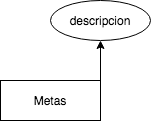
\includegraphics[scale=0.6]{er_lifegoals}
     \caption{Life Goals E-R Model}
\end{figure}
   
\section{Relational Model}
Life Goals Relational Model

\begin{figure}[h]
     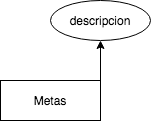
\includegraphics[scale=0.6]{er_lifegoals}
     \caption{Life Goals Relational Model}
\end{figure}

\end{document}

